\graphicspath{{./chapters/chapter4/}}
%\newtheorem{thm}{Theorem}
%\newtheorem{lem}[thm]{Lemma}
%\DeclareMathOperator*{\argmax}{arg\,max}
%\DeclareMathOperator*{\argmin}{arg\,min}
\newtheorem{theorem}{Theorem}[section]
\newtheorem{proposition}[theorem]{Proposition}
\newtheorem{lemma}[theorem]{Lemma}
\newtheorem{corollary}[theorem]{Corollary}
%\theoremstyle{definition}
\newtheorem{definition}[theorem]{Definition}
\newtheorem{assumption}[theorem]{Assumption}
%\theoremstyle{remark}
\newtheorem{remark}[theorem]{Remark}

\def\c{cr}
\def\hc{\hat{cr}}
\def\d{\Lambda}
\def\ind{\mathbbm{1}}
\def\oc{Online\_Cluster}
\def\mem{\mathcal M}
\def\E{\mathbb{E}}
\def\R{\mathbb{R}}
\def\O{\mathcal{O}}
\def\calP{\mathcal{P}}
\def\dc{Data\_Copy\_Detect}
\def\a{\kappa}
\def\hq{\widehat{q(B(x, r))}}
\def\alpaca{\epsilon}

\chapter{Data-Copying in Generative Models: A Formal Framework} 

\section{Introduction}

Deep generative models have shown impressive performance. However, given how large, diverse, and uncurated their training sets are, a big question is whether, how often, and how closely they are memorizing their training data. This question has been of considerable interest in generative modeling~\citep{lopez2016revisiting,XHYGSWK18} as well as supervised learning~\citep{BBFST21, Feldman20}. However, a clean and formal definition of memorization that captures the numerous complex aspects of the problem, particularly in the context of continuous data such as images, has largely been elusive.

For generative models,~\cite{MCD2020} proposed a formal definition of memorization called ``data-copying'', and showed that it was orthogonal to various prior notions of overfitting such as mode collapse~\citep{TT20}, mode dropping~\citep{YFWYC20}, and precision-recall~\citep{SBLBG18}. Specifically, their definition looks at three datasets -- a training set, a set of generated example, and an independent test set. Data-copying happens when the training points are considerably closer on average to the generated data points than to an independently drawn test sample. Otherwise, if the training points are further on average to the generated points than test, then there is underfitting. They proposed a three sample test to detect this kind of data-copying, and empirically showed that their test had good performance.

\begin{figure}[ht]
\centering
	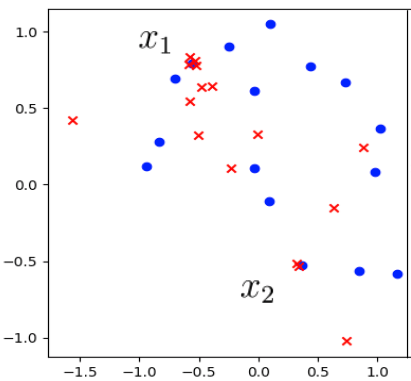
\includegraphics[width=.45\textwidth]{page_2_figure_yo.png}
	\caption{In this figure, the blue points are sampled from the halfmoons dataset (with Gaussian noise). The red points are sampled from a generated distribution that is a mixture of (40 \%) blatant data copier (that outputs a random subset of the training set), and (60 \%) a noisy underfit version of halfmoons. Although the generated distribution is clearly doing some form of copying at points $x_1$ and $x_2$, detecting this is challenging because of the canceling effect of the underfit points.}
	
	\label{fig:page_2_figure}
\end{figure}

However, despite its practical success, this method may not capture even blatant cases of memorization. To see this, consider the example illustrated in Figure \ref{fig:page_2_figure}, in which a generated model for the halfmoons dataset outputs one of its training points with probability $0.4$, and otherwise outputs a random point from an underfit distribution. When the test of~\cite{MCD2020} is applied to this distribution, it is unable to detect any form of data copying; the generated samples drawn from the underfit distribution are sufficient to cancel out the effect of the memorized examples. Nevertheless, this generative model is clearly an egregious memorizer as shown in points $x_1$ and $x_2$ of Figure \ref{fig:page_2_figure}.

This example suggests a notion of \textit{point-wise} data copying, where a model $q$ can be thought of as copying a given training point $x$. Such a notion would be able to detect $q$'s behavior nearby $x_1$ and $x_2$ regardless of the confounding samples that appear at a global level. This stands in contrast to the more global distance based approach taken in Meehan et. al. which is unable to detect such instances. Motivated by this, we propose an alternative point-by-point approach to defining data-copying.

We say that a generative model $q$  data-copies an individual training point, $x$, if it has an unusually high concentration in a small area centered at $x$. Intuitively, this implies $q$ is highly likely to output examples that are very similar to $x$. In the example above, this definition would flag $q$ as copying $x_1$ and $x_2$. 

To parlay this definition into a global measure of data-copying, we define the overall \textit{data-copying rate} as the total fraction of examples from $q$ that are copied from some training example. In the example above, this rate is $40\%$, as this is the fraction of examples that are blatant copies of the training data.

\begin{figure}[ht]
    \begin{subfigure}{0.31\textwidth}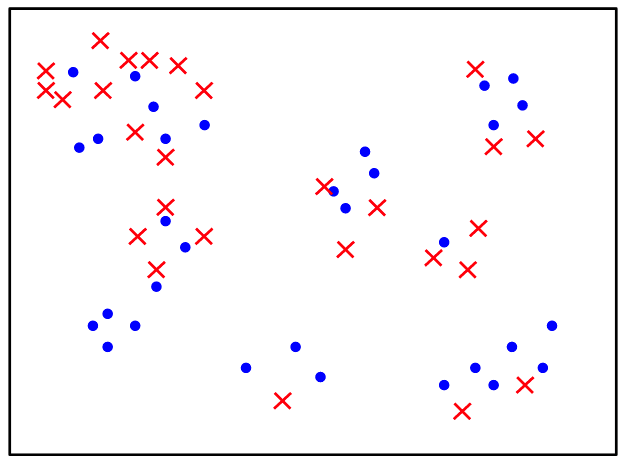
\includegraphics[width=\linewidth]{default.png}
    \end{subfigure}\hspace*{\fill}
	\begin{subfigure}{0.31\textwidth}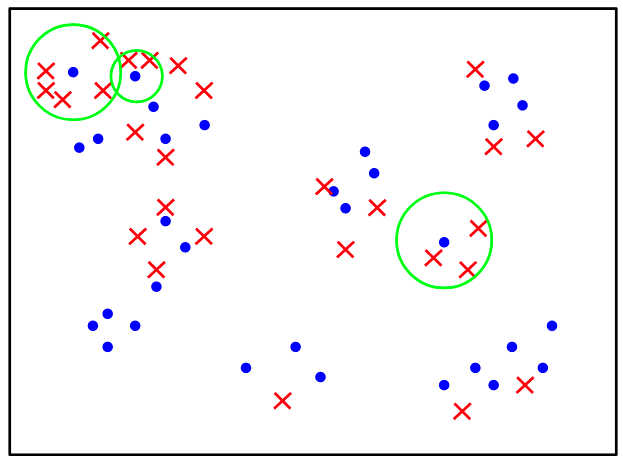
\includegraphics[width=\linewidth]{add_regions.png}
	\end{subfigure}\hspace*{\fill}
	\begin{subfigure}{0.31\textwidth}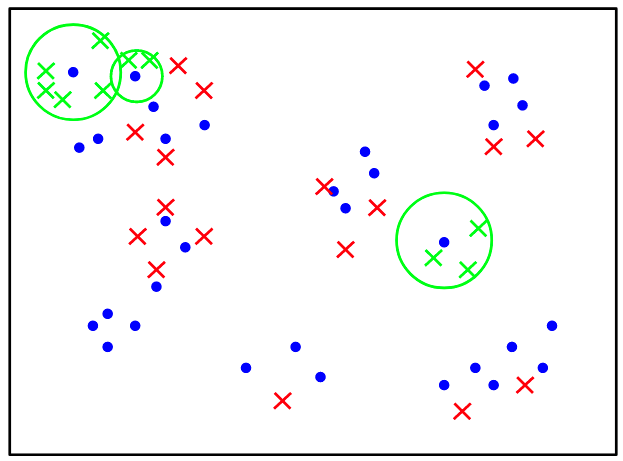
\includegraphics[width=\linewidth]{data_copy.png}
	\end{subfigure}
	\caption{In the three panels above, the blue points are a training sample from $p$, and the red points are generated examples from $q$. In the middle panel, we highlight in green regions that are defined to be \textit{data-copying regions}, as $q$ overrepresents them with comparison to $p$. In the third panel, we then color all points from $q$ that are considered to be copied green.}
	
	\label{fig:triptic}
\end{figure}

Next, we consider how to detect data-copying according to this definition. To this end, we provide an algorithm, \dc{}, that outputs an estimate for the overall data-copying rate. We then show that under a natural smoothness assumption on the data distribution, which we call \textit{regularity}, \dc{} is able to guarantee an accurate estimate of the total data-copying rate. We then give an upper bound on the amount of data needed for doing so. 

We complement our algorithm with a lower bound on the minimum amount of a data needed for data-copying detection. Our lower bound also implies that some sort of smoothness condition (such as regularity) is necessary for guaranteed data-copying detection; otherwise, the required amount of data can be driven arbitrarily high.

\subsection{Related Work}

Recently, understanding failure modes for generative models has been an important growing body of work e.g. \citep{SGZCRC16, RW18, SBLBG18}. However, much of this work has been focused on other forms of overfitting, such as mode dropping or mode collapse.

A more related notion of overfitting is \textit{memorization} \citep{lopez2016revisiting,XHYGSWK18, C18}, in which a model outputs exact copies of its training data. This has been studied in both supervised \citep{BBFST21, Feldman20} and unsupervised \citep{BGWC21, CHCW21} contexts. Memorization has also been considered in language generation models \cite{Carlini22}. 

The first work to explicitly consider the more general notion of \textit{data-copying} is \citep{MCD2020}, which gives a three sample test for data-copy detection. We include an empirical comparison between our methods in Section \ref{sec:experiments}, where we demonstrate that ours is able to capture certain forms of data-copying that theirs is not. 

Finally, we note that this work focuses on detecting natural forms of memorization or data-copying, that likely arises out of poor generalization, and is not concerned with detecting \textit{adversarial} memorization or prompting, such as in \cite{Carlini19}, that are designed to obtain sensitive information about the training set. This is reflected in our definition and detection algorithm which look at the specific generative model, and not the algorithm that trains it.  Perhaps the best approach to prevent adversarial  memorization is training the model with differential privacy~\cite{Dwork06}, which ensures that the model does not change much when one training sample changes. However such solutions come at an utility cost. 

\section{A Formal Definition of Data-Copying}

We begin with the following question: what does it mean for a generated distribution $q$ to copy a single training example $x$? Intuitively, this means that $q$ is guilty of overfitting $x$ in some way, and consequently produces examples that are very similar to it. 

However, determining what constitutes a `very similar'  generated example must be done contextually. Otherwise the original data distribution, $p$, may itself be considered a copier, as it will output points nearby $x$ with some frequency depending on its density at $x$. Thus, we posit that $q$ data copies training point $x$ if it has a significantly higher concentration nearby $x$ than $p$ does. We express this in the following definition. 

\begin{definition}\label{defn:data_copy}
Let $p$ be a data distribution, $S \sim p^n$ a training sample, and $q$ be a generated distribution trained on $S$. Let $x \in S$ be a training  point, and let $\lambda > 1$ and $0 < \gamma < 1$ be constants. A generated example $x' \sim q$ is said to be a \textbf{$(\lambda, \gamma)$-copy} of $x$ if there exists a ball $B$ centered at $x$ (i.e. $\{x': ||x' - x|| \leq r\}$) such that following hold:
\begin{itemize}
	\item $x' \in B$.
	\item $q(B) \geq \lambda p(B)$
	\item $p(B) \leq \gamma$
\end{itemize}
\end{definition}

Here $q(B)$ and $p(B)$ denote the probability mass assigned to $B$ by $p$ and $q$ respectively.

The parameters $\lambda$ and $\gamma$ are user chosen parameters that characterize data-copying. $\lambda$ represents the rate at which $q$ must overrepresent points close to $x$, with higher values of $\lambda$ corresponding to more egregious examples of data-copying. $\gamma$ represents the maximum size (by probability mass) of a region that is considered to be data-copying -- the ball $B$ represents all points that are ``copies" of $x$. Together, $\lambda$ and $\gamma$ serve as practitioner controlled knobs that characterize data-copying about $x$.

Our definition is illustrated in Figure \ref{fig:triptic} -- the training data is shown in blue, and generated samples are shown in red. For each training point, we highlight a region (in green) about that point in which the red density is much higher than the blue density, thus constituting data-copying. The intuition for this is that the red points within any ball can be thought of as ``copies" of the blue point centered in the ball.

Having defined data-copying with respect to a single training example, we can naturally extend this notion to the entire training dataset. We say that $x' \sim q$ is copied from training set $S$ if $x'$ is a $(\lambda,\gamma)$-copy of some training example $x \in S$. We then define the \textit{data-copy rate} of $q$ as the fraction of examples it generates that are copied from $S$. Formally, we have the following: 

\begin{definition}
Let $p, S, q, \lambda,$ and $\gamma$ be as defined in Definition \ref{defn:data_copy}. Then the \textbf{data-copy rate}, $\c\left(q, \lambda, \gamma\right)$ of $q$ (with respect to $p, S$) is the fraction of examples from $q$ that are $(\lambda, \gamma)$-copied. That is, $$\c\left(q, \lambda, \gamma\right) = \Pr_{x' \sim q}[q\text{ }(\lambda,\gamma)\text{-copies }x'].$$ In cases where $\lambda, \gamma$ are fixed, we use $\c_q = \c(q, \lambda, \gamma)$ to denote the data-copy rate.
\end{definition}

Despite its seeming global nature, $\c_q$ is simply an aggregation of the point by point data-copying done by $q$ over its entire training set. As we will later see, estimating $\c_q$ is often reduced to determining which subset of the training data $q$ copies. 

\subsection{Examples of data-copying}

We now give several examples illustrating our definitions. In all cases, we let $p$ be a data distribution, $S$, a training sample from $p$, and $q$, a generated distribution that is trained over $S$. 

\paragraph{The uniform distribution over $S$:} In this example, $q$ is an egregious data copier that memorizes its training set and randomly outputs a training point. This can be considered as the canonical \textit{worst} data copier. This is reflected in the value of $\c_q$ -- if $p$ is a continuous distribution with finite probability density, then for any $x \in S$, there exists a ball $B$ centered at $x$ for which $q(B) >> p(B)$. It follows that $q$ $(\lambda,\gamma)$- copies $x$ for all $x \in S$ which implies that $\c_q = 1$.

\paragraph{The perfect generative model: $q = p$:} In this case, $q(B) = p(B)$ for all balls, $B$, which implies that $q$ does not perform any data-copying (Definition \ref{defn:data_copy}). It follows that $\c_q = 0$, matching the intuition that $q$ does not data-copy at all.

\paragraph{Kernel Density Estimators:} Finally, we consider a more general situation, where $q$ is trained by a \textit{kernel density estimator} (KDE) over $S \sim p^n$. Recall that a kernel density estimator outputs a generated distribution, $q$, with pdf defined by $$q(x) = \frac{1}{n\sigma_n}\sum_{x_i \in S} K\left(\frac{x - x_i}{\sigma_n}\right).$$ Here, $K$ is a kernel similarity function, and $\sigma_n$ is the bandwidth parameter. It is known that for $\sigma_n = O(n^{-1/5})$, $q$ converges towards $p$ for sufficiently well behaved probability distributions. 

Despite this guarantee, KDEs intuitively appear to perform some form of data-copying -- after all they implicitly include each training point in memory as it forms a portion of their outputted pdf. However, recall that our main focus is in understanding \textit{overfitting} due to data-copying. That is, we view data-copying as a function of the outputted pdf, $q$, and not of the training algorithm used. 

To this end, for KDEs the question of data-copying reduces to the question of whether $q$ overrepresents areas around its training points. As one would expect, this occurs \textit{before} we reach the large sample limit. This is expressed in the following theorem.

\begin{theorem}\label{thm:KDE}
Let $1 < \lambda$ and $\gamma > 0$. Let $\sigma_n$ be a sequence of bandwidths and $K$ be any regular kernel function. For any $n > 0$ there exists a probability distribution $\pi$ with full support over $\R^d$ such that with probability at least $\frac{1}{3}$ over $S \sim \pi^n$, a KDE trained with bandwidth $\sigma_n$ and kernel function $K$ has data-copy rate $\c_q \geq \frac{1}{10}$.
\end{theorem}

This theorem completes the picture for KDEs with regards to data-copying -- when $n$ is too low, it is possible for the KDE to have a significant amount of data-copying, but as $n$ continues to grow, this is eventually smoothed out.

\paragraph{The Halfmoons dataset}

Returning to the example given in Figure \ref{fig:page_2_figure}, observe that our definition exactly captures the notion of data-copying that occurs at points $x_1$ and $x_2$. For even strict choices of $\lambda$ and $\gamma$, Definition \ref{defn:data_copy} indicates that the red distribution copies both $x_1$ and $x_2$. Furthermore, the data-copy rate, $\c_q$, is $40\%$ by construction, as this is the proportion of points that are outputted nearby $x_1$ and $x_2$.

\subsection{Limitations of our definition}\label{sec:limitations}

Definition \ref{defn:data_copy} implicitly assumes that the goal of the generator is to output a distribution $q$ that approaches $p$ in a mathematical sense; a perfect generator would output $q$ so that $q(M) = p(M)$ for all measurable sets. In particular, instances where $q$ outputs examples that are far away from the training data are considered completely irrelevant in our definition.

This restriction prevents our definition from capturing instances in which $q$ memorizes its training data and then applies some sort of transformation to it. For example, consider an image generator that applies a color filter to its training data. This would not be considered a data-copier as its output would be quite far from the training data in pixel space. Nevertheless, such a generated distribution can be very reasonably considered as an egregious data copier, and a cursory investigation between its training data and its outputs would reveal as much. 

The key difference in this example is that the generative algorithm is no longer trying to closely approximate $p$ with $q$ -- it is rather trying to do so in some kind of transformed space. Capturing such interactions is beyond the scope of our paper, and we firmly restrict ourselves to the case where a generator is evaluated based on how close $q$ is to $p$ with respect to their measures over the input space. 

\section{Detecting data-copying}

Having defined $\c_q$, we now turn our attention towards \textit{estimating it.} To formalize this problem, we will require a few definitions. We begin by defining a generative algorithm.

\begin{definition}
A \textbf{generative algorithm}, $A$, is a potentially randomized algorithm that outputs a distribution $q$ over $\R^d$ given an input of training points, $S \subset \R^d$. We denote this relationship by $q \sim A(S)$.
\end{definition}

This paradigm captures most typical generative algorithms including both non-parametric methods such as KDEs and parametric methods such as variational autoencoders.

As an important distinction, in this work we define data-copying as a property of the generated distribution, $q$, rather than the generative algorithm, $A$. This is reflected in our definition which is given solely with respect to $q, S,$ and $p$. For the purposes of this paper, $A$ can be considered an arbitrary process that takes $S$ and outputs a distribution $q$. We include it in our definitions to emphasize that while $S$ is an i.i.d sample from $p$, it is \textit{not} independent from $q$. 

Next, we define a \textit{data-copying detector} as an algorithm that estimates $\c_q$ based on access to the training sample, $S$, along with the ability to draw any number of samples from $q$. The latter assumption is quite typical as sampling from $q$ is a purely computational operation. We do not assume any access to $p$ beyond the training sample $S$. Formally, we have the following definition.

\begin{definition}\label{def:data_copy_detector}
A \textbf{data-copying detector} is an algorithm $D$ that takes as input a training sample, $S \sim p^n$, and access to a sampling oracle for $q \sim A(S)$ (where $A$ is an arbitrary generative algorithm). $D$ then outputs an estimate, $D(S, q) = \hc_q$, for the data-copy rate of $q$. 
\end{definition}

Naturally, we assume $D$ has access to $\lambda, \gamma >0$ (as these are practitioner chosen values), and by convention don't include $\lambda, \gamma$ as formal inputs into $D$. 

The goal of a data-copying detector is to provide accurate estimates for $\c_q$. However, the precise definition of $\c_q$ poses an issue: data-copy rates for varying values of $\lambda$ and $ \gamma$ can vastly differ. This is because $\lambda, \gamma$ act as thresholds with everything above the threshold being counted, and everything below it being discarded. Since $\lambda, \gamma$ cannot be perfectly accounted for, we will require some tolerance in dealing with them. This motivates the following.

\begin{definition}\label{defn:approx_data_copy_rate}
Let $0 < \alpaca$ be a tolerance parameter. Then the \textbf{approximate data-copy rates}, $\c_q^{-\alpaca}$ and $\c_q^\alpaca$, are defined as the values of $\c_q$ when the parameters $(\lambda, \gamma)$ are shifted by a factor of $(1+\alpaca)$ to respectively decrease and increase the copy rate. That is, $$\c_q^{-\alpaca} = \c\left(q, \lambda (1+\alpaca), \gamma (1+\alpaca)^{-1}\right),$$ $$\c_q^{\alpaca} = \c\left(q, \lambda (1+\alpaca)^{-1}, \gamma (1+\alpaca)\right).$$
\end{definition}

The shifts in $\lambda$ and $\gamma$ are chosen as above because increasing $\lambda$ and decreasing $\gamma$ both reduce $\c_q$ seeing as both result in more restrictive conditions for what qualifies as data-copying. Conversely, decreasing $\lambda$ and increasing $\gamma$ has the opposite effect. It follows that $$\c_q^{-\alpaca} \leq \c_q \leq \c_q^{\alpaca},$$ meaning that $\c_q^{-\alpaca}$ and $\c_q^{\alpaca}$ are lower and upper bounds on $\c_q$. 

In the context of data-copying detection, the goal is now to estimate $\c_q$ in comparison to $\c_q^{\pm \alpaca}$. We formalize this by defining \textit{sample complexity} of a data-copying detector as the amount of data needed for accurate estimation of $\c_q$. 

\begin{definition}\label{def:sample_complexity}
Let $D$ be a data-copying detector and $p$ be a data distribution. Let $\epsilon, \delta > 0$ be standard tolerance parameters. Then $D$ has \textbf{sample complexity}, $m_p(\epsilon, \delta)$, with respect to $p$ if for all $n \geq m_p(\epsilon, \delta)$, $\lambda >1$, $0 < \gamma < 1$, and generative algorithms $A$, with probability at least $1 - \delta$ over $S \sim p^n$ and $q \sim A(S)$, $$\c_q^{-\alpaca} - \epsilon \leq D(S, q) \leq \c_q^{\alpaca} + \epsilon.$$
\end{definition}

Here the parameter $\epsilon$ takes on a somewhat expanded as it is both used to additively bound our estimation of $\c_q$ and to multiplicatively bound $\lambda$ and $\gamma$.

Observe that there is no mention of the number of calls that $D$ makes to its sampling oracle for $q$. This is because samples from $q$ are viewed as \textit{purely computational}, as they don't require any natural data source. In most cases, $q$ is simply some type of generative model (such as a VAE or a GAN), and thus sampling from $q$ is a matter of running the corresponding neural network.

\section{Regular Distributions}\label{sec:regular_dist}

Our definition of data-copying (Definition \ref{defn:data_copy}) motivates a straightforward point by point method for data-copying detection, in which for every training point, $x_i$, we compute the largest ball $B_i$ centered at $x_i$ for which $q(B_i) \geq \lambda p(B_i)$ and $p(B_i) \leq \gamma$. Assuming we compute these balls accurately, we can then query samples from $q$ to estimate the total rate at which $q$ outputs within those balls, giving us our estimate of $\c_q$.

The key ingredient necessary for this idea to work is to be able to reliably estimate the masses, $q(B)$ and $p(B)$ for any ball in $\R^d$. The standard approach to doing this is through \textit{uniform convergence}, in which large samples of points are drawn from $p$ and $q$ (in $p$'s case we use $S$), and then the mass of a ball is estimated by counting the proportion of sampled points within it. For balls with a sufficient number of points (typically $O( d\log n)$), standard uniform convergence arguments show that these estimates are reliable.

However, this method has a major pitfall for our purpose -- in most cases the balls $B_i$ will be very small because data-copying intrinsically deals with points that are very close to a given training point. While one might hope that we can simply ignore all balls below a certain threshold, this does not work either, as the sheer number of balls being considered means that their union could be highly non-trivial. 

To circumvent this issue, we will introduce an interpolation technique that estimates the probability mass of a small ball by scaling down the mass of a sufficiently large ball with the same center. While obtaining a general guarantee is impossible -- there exist pathological  distributions that drastically change their behavior at small scales -- it turns out there is a relatively natural condition under which such interpolation will work. We refer to this condition as \textit{regularity,} which is defined as follows.

\begin{definition}\label{def:regular}
Let $k> 0$ be an integer. A probability distribution $p$ is \textbf{$k$-regular} the following holds. For all $\alpaca > 0$, there exists a constant $0 < p_\alpaca \leq 1$ such that for all $x$ in the support of $p$, if $0 < s < r$ satisfies that $p(B(x, r)) \leq p_\alpaca$, then $$\left(1+\frac{\alpaca}{3}\right)^{-1}\frac{r^k}{s^{k}} \leq \frac{p(B(x, r))}{p(B(x, s))} \leq \left(1+\frac{\alpaca}{3}\right)\frac{r^k}{s^{k}}.$$ Finally, a distribution is \textbf{regular} if it is $k$-regular for some integer $k > 0$. 
\end{definition}

Here we let $B(x, r) = \{x': ||x - x'|| \leq r\}$ denote the closed $\ell_2$ ball centered at $x$ with radius $r$. 

The main intuition for a $k$-regular distribution is that at a sufficiently small scale, its probability mass scales with distance according to a power law, determined by $k$. The parameter $k$ dictates how the probability density behaves with respect to the distance scale. In most common examples, $k$ will equal the \textit{intrinsic dimension}  of $p$.

As a technical note, we use an error factor of $\frac{\alpaca}{3}$ instead of $\alpaca$ for technical details that enable cleaner statements and proofs in our results (presented later). 

\subsection{Distributions with Manifold Support}

We now give an important class of $k$-regular distributions.

\begin{proposition}\label{prop:manifold_works}
Let $p$ be a probability distribution with support precisely equal to a compact $k$ dimensional sub-manifold (with or without boundary) of $\R^d$, $M$. Additionally, suppose that $p$ has a continuous density function over $M$. Then it follows that $p$ is $k$-regular.
\end{proposition}

Proposition \ref{prop:manifold_works} implies that most data distributions that adhere to some sort of manifold-hypothesis will also exhibit regularity, with the regularity constant, $k$, being the intrinsic dimension of the manifold.

\subsection{Estimation over regular distributions}

We now turn our attention towards designing estimation algorithms over regular distributions, with our main goal being to estimate the probability mass of arbitrarily small balls. We begin by first addressing a slight technical detail -- although the data distribution $p$ may be regular, this does not necessarily mean that the regularity constant, $k$, is known. Knowledge of $k$ is crucial because it determines how to properly interpolate probability masses from large radius balls to smaller ones. 

Luckily, estimating $k$ turns out to be an extremely well studied task, as for most probability distributions, $k$ is a measure of the \textit{intrinsic dimension}. Because there is a wide body of literature in this topic, we will assume from this point that $k$ has been correctly estimated from $S$ using any known algorithm for doing so (for example \cite{BJPR22}). Nevertheless, for completeness, we provide an algorithm with provable guarantees for estimating $k$ (along with a corresponding bound on the amount of needed data) in Appendix \ref{sec:estimating_alpha}.

We now return to the problem of $p(B(x, r))$ for a small value of $r$, and present an algorithm, $Est(x, r, S)$ (Algorithm \ref{alg:estimate}), that estimates $p(B(x, r))$ from an i.i.d sample $S \sim p^n$.

\begin{algorithm}
   \caption{$Est(x, r, S)$}
   \label{alg:estimate}

   \DontPrintSemicolon
   
	$n \leftarrow |S|$\;
	
   $b \leftarrow O\left(\frac{d \ln \frac{n}{\delta}}{\epsilon^2} \right)$\;
   
   $r_* = \min \{s > 0, |S \cap B(x, s)| = b\}$.\;
   
   \uIf{$r_* > r$}{
   Return $\frac{br^k}{nr_*^k}$\;
   }
   \uElse {
	Return $\frac{|T \cap B(x, r)|}{n}$\;
	}

\end{algorithm}

$Est$ uses two ideas: first, it leverages standard uniform convergence results to estimate the probability mass of all balls that contain a sufficient number of training examples. This is what leads to the specific value of $b$ that is chosen. Second, it estimates the mass of smaller balls by interpolating from its estimates from larger balls. The $k$-regularity assumption is crucial for this second step as it is the basis on which such interpolation is done. 

$Est$ has the following performance guarantee, which follows from standard uniform convergence bounds and the definition of $k$-regularity. 
\begin{proposition}\label{prop:est_works}
Let $p$ be a regular distribution, and let $\alpaca >0$ be arbitrary. Then if $n = O\left(\frac{d\ln\frac{d}{\delta \alpaca p_\alpaca}}{\alpaca^2 p_\alpaca}\right)$ with probability at least $1 - \delta$ over $S \sim p^n$, for all $x \in \R^d$ and $r > 0$, $$\left(1+\frac{\alpaca}{2}\right)^{-1}\leq \frac{Est(x, r, S)}{p(B(x, r))} \leq \left(1+\frac{\alpaca}{2}\right).$$
\end{proposition}

\section{A Data-copy detecting algorithm}

\begin{algorithm}    

\caption{$DataCopyDetect(S, q, m)$}
\label{alg:main}   

   \DontPrintSemicolon
   
   $m \leftarrow O\left(\frac{dn^2\ln \frac{nd}{\delta\epsilon}}{\epsilon^4}\right)$\;
   
   Sample $T \sim q^m$\;
   
   $\{x_1, x_2, \dots, x_n\} \leftarrow S$\;
   
   $\{z_1, z_2, \dots, z_m\} \leftarrow T$\;

	\For{$i = 1, \dots, n$}{
	
	Let $p_i(r)$ denote $Est(x_i, r, S)$\;
	
	Let $q_i(r)$ denote $\frac{|B(x_i, r) \cap T|}{m}$\;
	
	$radii \leftarrow \{||z - x_i||: z \in T\} \cup \{0\}$\;
	
	$radii \leftarrow \{r: p_i(r) \leq \gamma, r \in radii\}$\;

	$r_i^* \leftarrow \max \{r: q_i(r) \geq \lambda p_i(r), r \in radii\}$\;
		
	}
	Sample $U \sim q^{20/\epsilon^2}$\;
	$V \leftarrow U \cap \left(\bigcup_{i=1}^n B(x_i, r_i^*)\right)$\;
	Return $\frac{|V|}{|U|}$.\;
	
	

\end{algorithm}


We now now leverage our subroutine, $Est$, to construct a data-copying detector, $Data\_Copy\_Detect$ (Algorithm \ref{alg:main}), that has bounded sample complexity when $p$ is a regular distribution. Like all data-copying detectors (Definition \ref{def:data_copy_detector}), $Data\_Copy\_Detect$ takes as input the training sample $S$, along with the ability to sample from a generated distribution $q$ that is trained from $S$. It then performs the following steps:
\begin{enumerate}
	\item (line 1) Draw an i.i.d sample of $m = O\left(\frac{dn^2\ln \frac{nd}{\delta\epsilon}}{\epsilon^4}\right)$ points from $q$. 
	\item (lines 6 - 10) For each training point, $x_i$, determine the largest radius $r_i$ for which 
	\begin{equation*}
	\begin{split}
	&\frac{|B(x_i, r_i) \cap T|}{m} \geq \lambda Est(x_i, r_i ,S), \\ 
	&Est(x_i, r_i , S) \leq \gamma.
	\end{split}
	\end{equation*}
	\item (lines 12 - 13) Draw a fresh sample of points from $U \sim q^{O(1/\epsilon^2)}$, and use it to estimate the probability mass under $q$ of $\cup_{i=1}^n B(x_i, r_i)$.
\end{enumerate}

In the first step, we draw a \textit{large} sample from $q$. While this is considerably larger than the amount of training data we have, we note that samples from $q$ are considered free, and thus do not affect the sample complexity. The reason we need this many samples is simple -- unlike $p$, $q$ is not necessarily regular, and consequently we need enough points to properly estimate $q$ around every training point in $S$.

The core technical details of $\dc{}$ are contained within step 2, in which data-copying regions surrounding each training point, $x_i$, are found. We use $Est(x, r, S)$ and $\frac{|B(x, r) \cap T|}{m}$ as proxies for $p$ and $q$ in Definition \ref{defn:data_copy}, and then search for the maximal radius $r_i$ over which the desired criteria of data-copying are met for these proxies.  

The only difficulty in doing this is that this could potentially require checking an infinite number of radii, $r_i$. Fortunately, this turns out not to be needed because of the following observation -- we only need to check radii at which a new point from $T$ is included in the estimation $q_i(r)$. This is because these our estimation for $q_i(r)$ does not change between them meaning that our estimate of the ratio between $q$ and $p$ is maximal nearby these points. 

Once we have computed $r_i$, all that is left is to estimate the data-copy rate by sampling $q$ once more to find the total mass of data-copying region, $\cup_{i=1}^n B(x_i, r_i)$. 

\subsection{Performance of Algorithm \ref{alg:main}}

We now show that given enough data, $\dc{}$ provides a close approximation of $\c_q$. 

\begin{theorem}\label{thm:upper_bound5}
$\dc{}$ is a data-copying detector (Definition \ref{def:data_copy_detector}) with sample complexity at most $$m_p(\epsilon, \delta) = O\left(\frac{d\ln\frac{d}{\delta\alpaca p_\alpaca}}{\alpaca^2 p_\alpaca}\right),$$ for all regular distributions, $p$. 
\end{theorem}

Theorem \ref{alg:main} shows that our algorithm's sample complexity has standard relationships with the tolerance parameters, $\epsilon$ and $\delta$, along with the input space dimension $d$. However, it includes an additional factor of $\frac{1}{p_\epsilon}$, which is a distribution specific factor measuring the regularity of the probability distribution. Thus, our bound cannot be used to give a bound on the amount of data needed without having a bound on $p_\epsilon$. 

We consequently view our upper bound as more akin to a convergence result, as it implies that our algorithm is guaranteed to converge as the amount of data goes towards infinity.

\subsection{Applying Algorithm \ref{alg:main} to Halfmoons}\label{sec:experiments}

We now return to the example presented in Figure \ref{fig:halfmoons} and empirically investigate the following question: is our algorithm able to outperform the one given in \cite{MCD2020} over this example? 

To investigate this, we test both algorithms over a series of distributions by varying the parameter $\rho$, which is the proportion of points that are ``copied." Figure \ref{fig:halfmoons} demonstrates a case in which $\rho = 0.4$. Additionally, we include a parameter, $c$, for \cite{MCD2020}'s algorithm which represents the number of clusters the data is partitioned into (with $c$-means clustering) prior to running their test. Intuitively, a larger number of clusters means a better chance of detecting more localized data-copying.

The results are summarized in the following table where we indicate whether the algorithm determined a statistically significant amount of data-copying over the given generated distribution and corresponding training dataset. Full experimental details can be found in Sections \ref{sec:app_experiments} and \ref{sec:experiments_details} of the appendix.

\begin{table}[h]
\caption{Statistical Significance of data-copying Rates over Halfmoons} \label{results_main}
\begin{center}
\begin{tabular}{ |c||c|c|c|c|c| } 
 \hline
 \textbf{Algo} & $\mathbf{q = p}$ & $\mathbf{\rho = 0.1}$ & $\mathbf{0.2}$ & $\mathbf{0.3}$ & $\mathbf{0.4}$ \\ 
 \hline
 \hline
 \textbf{Ours} & \color{blue}no & \color{red}yes & \color{red}yes & \color{red}yes & \color{red}yes \\ 
 \hline
 $\mathbf{c=1}$ & \color{blue}no & \color{blue}no & \color{blue}no & \color{blue}no & \color{blue}no \\ 
 \hline
 $\mathbf{c=5}$ & \color{blue}no & \color{blue}no & \color{blue}no & \color{blue}no & \color{red}yes \\ 
 \hline
 $\mathbf{c=10}$ & \color{blue}no & \color{blue}no & \color{blue}no & \color{blue}no & \color{red}yes \\ 
 \hline
 $\mathbf{c=20}$ & \color{blue}no & \color{blue}no& \color{blue}no & \color{red}yes & \color{red}yes\\ 
 \hline
\end{tabular}
\end{center}
\end{table}

As the table indicates, our algorithm is able to detect statistically significant data-copying rates in all cases it exists. By contrast, \cite{MCD2020}'s test is only capable of doing so when there is a large data-copy rate and when the number of clusters, $c$, is quite large.

\section{Is smoothness necessary for data copying detection?}\label{sec:lower_bound}

Algorithm \ref{alg:main}'s performance guarantee requires that the input distribution, $p$, be regular (Definition \ref{def:regular}). This condition is essential for the algorithm to successfully estimate the probability mass of arbitrarily small balls. Additionally, the parameter, $p_\epsilon$, plays a key role as it serves as a measure of how ``smooth" $p$ is with larger values implying a higher degree of smoothness. 

This motivates a natural question -- can data copying detection be done over unsmooth data distributions? Unfortunately, the answer turns out to be no. In the following result, we show that if the parameter, $p_\epsilon$ is allowed to be arbitrarily small, then this implies that for any data-copy detector, there exists $p$ for which the sample complexity is arbitrarily large.

\begin{theorem}\label{thm:lower_bound5}
Let $B$ be a data-copying detector. Let $\epsilon = \delta = \frac{1}{3}$. Then, for all integers $\a > 0$, there exists a probability distribution $p$ such that $\frac{1}{9\a} \leq p_\alpaca \leq \frac{1}{\a}$, and $m_p(\epsilon, \delta) \geq \a$, implying that $$m_p(\epsilon, \delta) \geq \Omega\left(\frac{1}{p_\epsilon}\right).$$
\end{theorem}

Although Theorem \ref{thm:lower_bound5} is restricted to regular distributions, it nevertheless demonstrates that a bound on smoothness is essential for data copying detection. In particular, non-regular distributions (with no bound on smoothness) can be thought of as a degenerate case in which $p_\epsilon = 0$. 

Additionally, Theorem \ref{thm:lower_bound5} provides a lower bound that complements the Algorithm \ref{alg:main}'s performance guarantee (Theorem \ref{thm:upper_bound5}). Both bounds have the same dependence on $p_\alpaca$ implying that our algorithm is optimal at least in regards to $p_\alpaca$. However, our upper bound is significantly larger in its dependence on $d$, the ambient dimension, and $\alpaca$, the tolerance parameter itself. 

While closing this gap remains an interesting direction for future work, we note that the existence of a gap isn't too surprising for our algorithm, $\dc{}$. This is because $\dc{}$ essentially relies on manually finding the entire region in which data-copying occurs, and doing this requires precise estimates of $p$ at all points in the training sample.  

Conversely, detecting data-copying only requires an \textit{overall} estimate for the data-copying rate, and doesn't necessarily require finding all of the corresponding regions. It is plausible that more sophisticated techniques might able to estimate the data-copy rate \textit{without} directly finding these regions.

\section{Conclusion}

In conclusion, we provide a new modified definition of ``data-copying'' or generating memorized training samples for generative models that addresses some of the failure modes of previous definitions~\cite{MCD2020}. We provide an algorithm for detecting data-copying according to our definition, establish performance guarantees, and show that at least some smoothness conditions are needed on the data distribution for successful detection. 

With regards to future work, one important direction is in addressing the limitations discussed in section \ref{sec:limitations}. Our definition and algorithm are centered around the assumption that the goal of a generative model is to output $q$ that is close to $p$ in a mathematical sense. As a result, we are unable to handle cases where the generator tries to generate \textit{transformed} examples that lie outside the support of the training distribution. For example, a generator restricted to outputting black and white images (when trained on color images) would remain completely undetected by our algorithm regardless of the degree with which it copies its training data. To this end, we are very interested in finding generalizations of our framework that are able to capture such broader forms of data-copying. 








%\input{chapters/chapter1/macros}
%\input{chapters/chapter1/introduction}
%\input{chapters/chapter1/related}
%\input{chapters/chapter1/definition}
%\input{chapters/chapter1/quantifying}
%\input{chapters/chapter1/visualizing}
%\input{chapters/chapter1/mitigation}